\subsection{The TorPath Protocol}

\subsubsection{Overview}

We introduce the TorPath protocol for assigning Tor circuits to clients. It
overrides Tor directory servers with \textit{assignment servers}, which form
decentralized \textit{consensus groups}. The protocol guarantees that no
participant on a circuit can identify all other participants, and that each
circuit includes a publicly verifiable signature. We use TorPath to ``sign''
each TorCoin, so that anyone can verify its authenticity.

\subsubsection{Requirements}

The TorPath protocol adheres to the following constraints:

\begin{itemize}   
\item No client can generate its own circuit.   
\item Every circuit has a unique, publicly-verifiable signature.   
\item No client can know the circuit of another client. 
\end{itemize}

\subsubsection{Protocol Description}

\paragraph{Group Formation}

A consensus group is formed when a majority of the Assignment Servers come
together to assign circuits to clients. Thus, if there are 10 Assignment Servers
in the world, atleast 6 of them must collectively form a group.

The steps in group formation are: 
\begin{enumerate} 
\item Some Assignment Servers come together to form a group. Each server shares 
its own public key with all the others. 
\item Clients connect to an assignment server that is accepting clients and 
download the public keys of all the assignment servers in the group.
\item Relays connect to an assignment server and download the public
keys of all assignment servers in the group. 
\item Clients generate a temporary public and private key-pair. The public key 
is then onion-wrapped with all the servers' public keys and sent to the server.
\end{enumerate}

\paragraph{Verifiable Shuffle} 
In most cases, the number of available relays will be less than that of clients 
in a group. The server will then ask each relay to generate some number of 
keypairs, such that the total number of such keypairs is equal to the number of 
clients. The public keys are then onion-hashed with the public keys of all the 
servers and sent to the servers.

The servers then perform a series of verifiable shuffles (eg. using the Neff
Shuffle) on each kind of key: Client Keys, Entry relay keys, exit relay keys and 
middle relay keys.

The input and output of the Shuffle is described in FIGURE. We may represent the
results of the shuffle as a $n \times 4$ matrix $M$, with each row representing 
a client and its three relays. This output matrix is also publicly published in 
a log and signed by all the servers participating in the group.

\paragraph{Path Lookup}
Once the shuffle is completed and published, all clients and relays can look up
their own keys in their respective columns. Using this information, they send 
their IP Address information encrypted in the following format:

For each row $i$ in the matrix $M$:

The client sends to the server:

($K_{ci}$, {$IP_{ci}$ hashed with the public key of its entry relay})

The entry relay sends:

($K_{ei}$, {$IP_{e1}$ hashed with the public key of its corresponding client}, 
{$IP_{e1}$ hashed with the public key of its corresponding middle relay})

Similarly, the middle and exit relays send:

($K_{mi}$, {$IP_{mi}$ hashed with the public key of corresponding entry relay}, 
{$IP_{m1}$ hashed with the public key of corresponding exit relay})

($K_{xi}$, {$IP_{xi}$ hashed with the public key of corresponding middle relay})

\begin{figure}
  \centering
    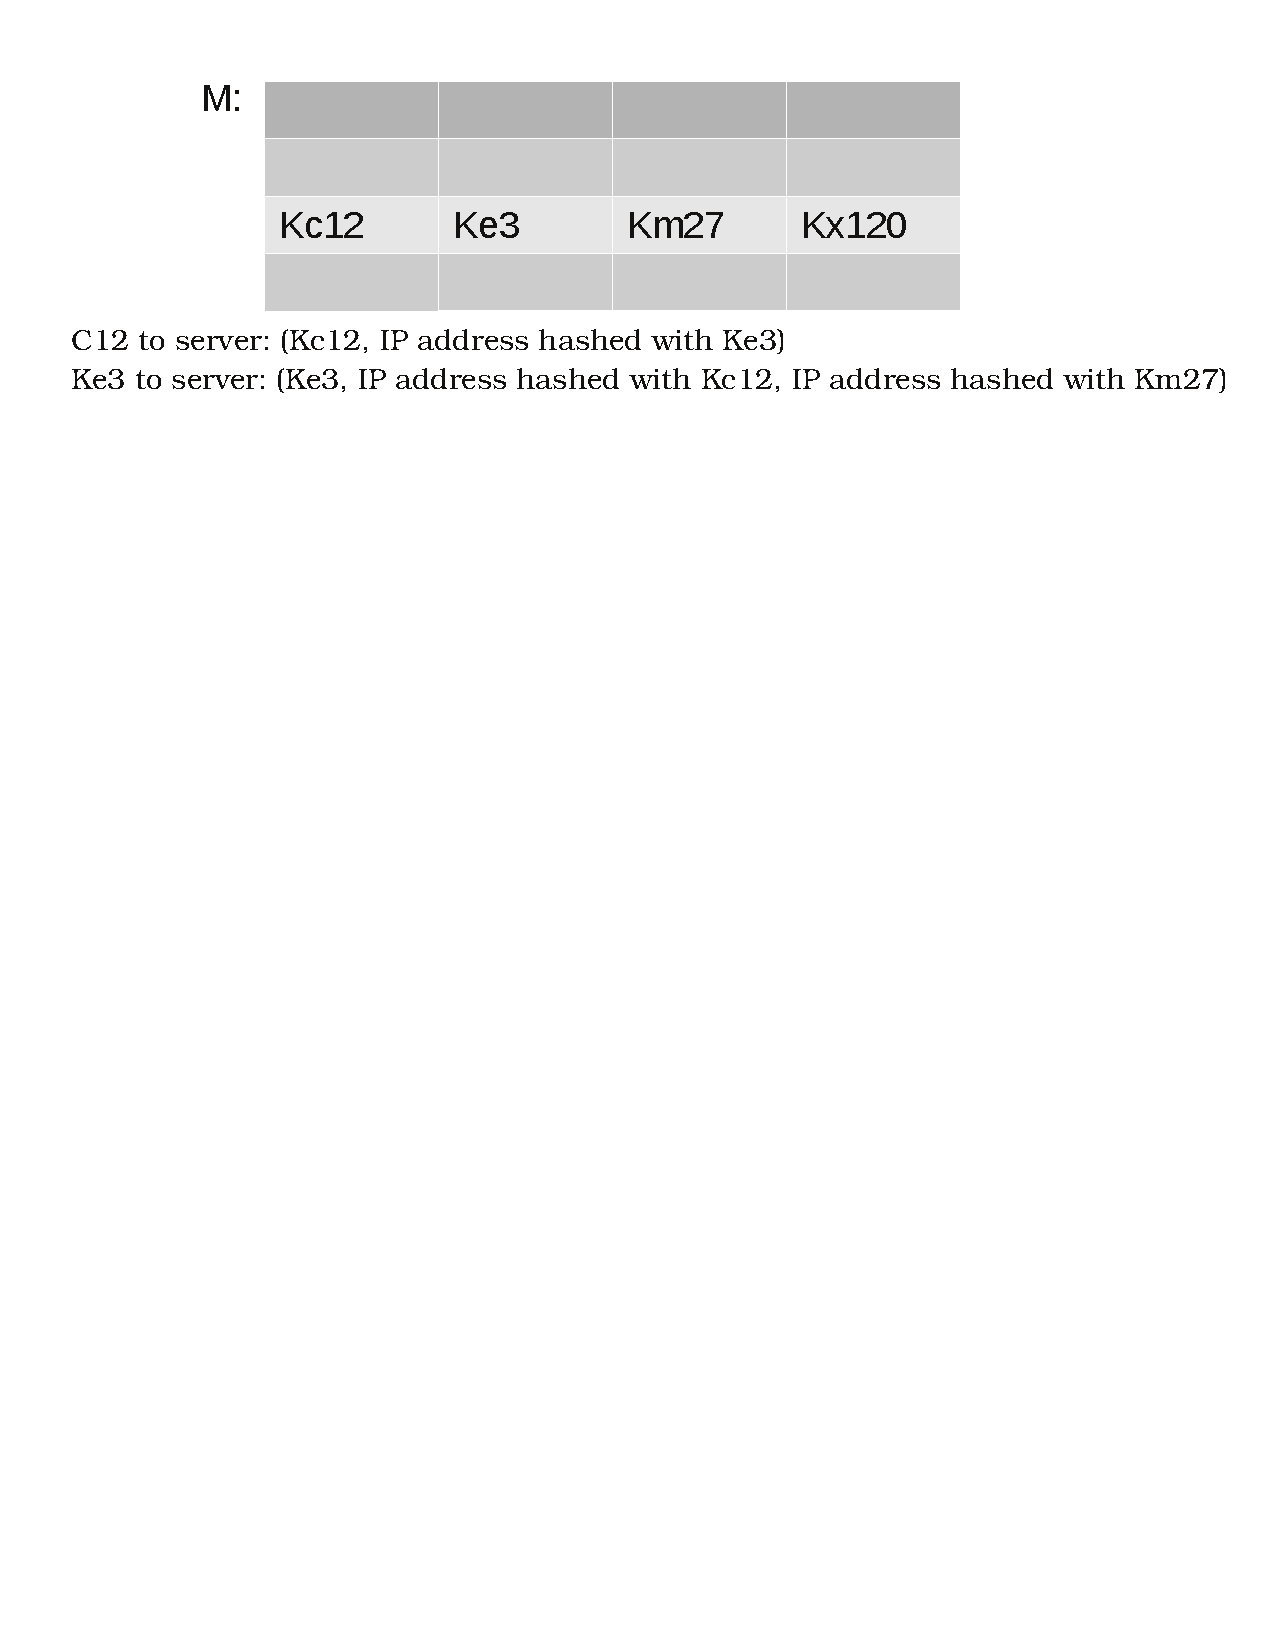
\includegraphics[scale=0.5]{address_lookup.pdf}
  \caption{An Example Path Lookup}
\end{figure}

These tuples are shuffled by the servers again. Each client and relay can then 
decrypt the IP address of their neighbours using their own public key.

The clients now have a circuit which they can use to communicate using the Tor 
protocol.

\paragraph{Route Signature}
The Route Signature of the ith circuit in a shuffle is the product of the keys
in row i of the matrix:
$RS_i = M_{i0} \times M_{i1} \times M_{i2} \times M_{i3}$
This key, using El Gamal encryption, can be used to verify the  proof-of-work.

\subsubsection{Circuit Anonymity} 
The TorPath protocol guarantees that no single server can be aware of the entire
circuit of any client. 


% % Next we will descibe the consensus groups and Neff shuffle in more detail.

% % \begin{figure}[H] %   \centering %
% 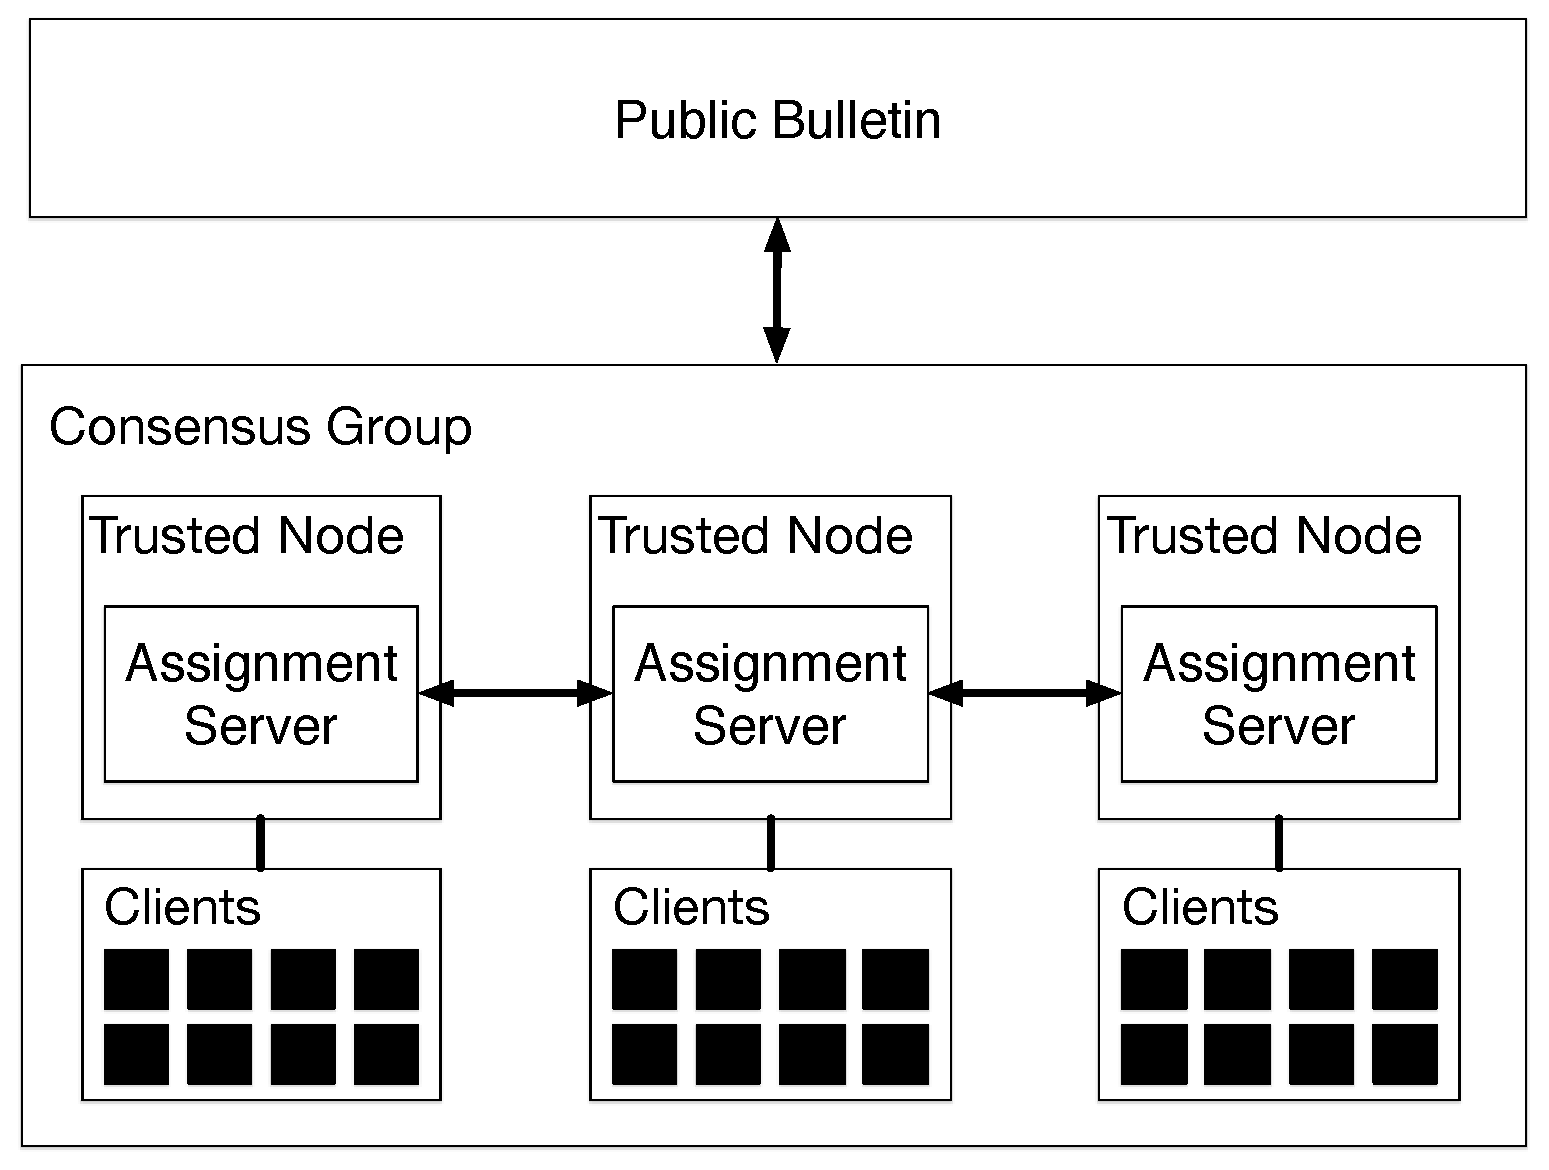
\includegraphics[scale=0.3]{torpath_grouping.pdf} %   \caption{TorPath Consensus
% Group Formation.} % \end{figure}

% % \subsubsection{Group Formation} % An assignment server joins a group when it
% reaches a sufficient number of clients. In practice, we expect the number to be
% modulated so that groups are being created every 10 seconds or so. To ensure
% diversity, groups must include a majority of the assignment servers on the
% network. For example, if there are ten of assignment servers on the entire
% network, a consensus group requires at least six.

% % Once a consensus group exists, it splits into three decentralized shuffle
% % sets, each responsible for assigning a different relay to clients. An
% % $n$-client shuffle set has $n$ rows, each pointing to a possible relay. For
% % example, shuffle sets $s_0$, $s_1$, and $s_2$ could be responsible for
% % assigning entry, middle, and exit relays to clients.

% % \subsubsection{Neff Shuffles for Circuit Assignment} % Each shuffle set runs a
% Neff shuffle ~\cite{neff2001verifiable} to shuffle its list of $n$ relays, so
% that it can assign each relay $i$ to client $i$. Each client receives a tuple
% $(r_0, r_1, r_2, s)$ specifying the address of entry, middle, and exit relays,
% along with a circuit signature.

% % \begin{figure} %   \centering %
% 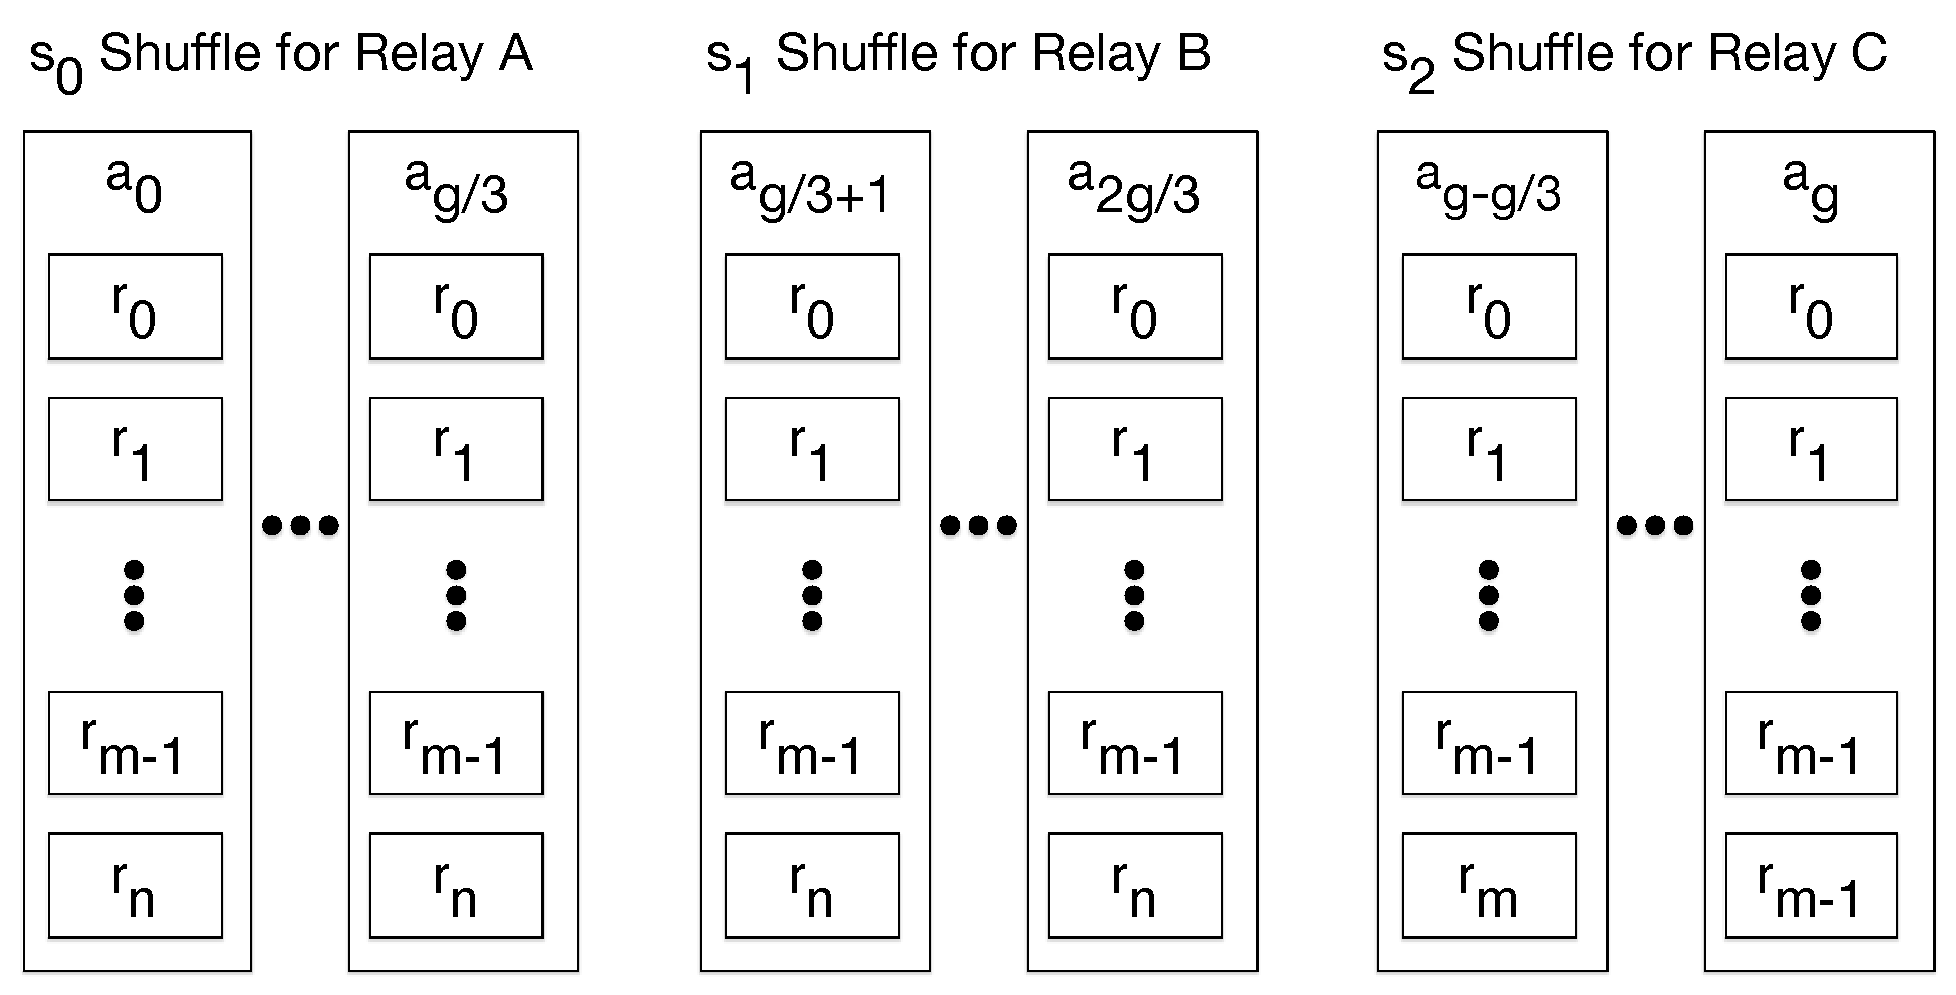
\includegraphics[scale=0.3]{torpath_shufflesets.pdf} %   \caption{Each Shuffle
% Set carries out its own Neff shuffle to determine one part of the path.} %
% \end{figure}

% % \subsubsection{TorCoin Verification} % Assignment servers input circuit
% signatures into a cryptographic accumulator, and publish that list of
% accumulators. Anyone can verify that a circuit existed at least once, simply by
% searching for a signature.

% % \subsubsection{Decoupled Protocol} % The TorPath protocol only replaces
% directory servers. Therefore, implementing it does not require modifying any Tor
% code. So clients can use the TorPath protocol for circuit assignment then
% communicate using the existing Tor protocol.
